% !TEX root = main-msc.tex
% !TEX encoding = UTF-8 Unicode
% !TEX TS-program = pdflatexmk
% !TEX spellcheck = en-US
% !BIB program = biber

%%%%%%%%%%%%%%%%%%%%%%%%%%%%%%%%%%%%%%%%%%%%%%%%%%%%%%%%%%%%%%%
%% UHH LT THESIS TEMPLATE based on the OXFORD THESIS TEMPLATE
%% see main.tex for explanations and options

%%%%% CHOOSE PAGE LAYOUT
% PDF output (ie equal margins, no extra blank pages, for online publication):
\documentclass[hidelinks, a4paper, nobind, msc]{conf/uhhltthesis}

% Your full degree name.
\degree{Master of Science (M.\ Sc.)}

% outsource configurations
% !TEX root = ../main.tex
% !TEX encoding = UTF-8 Unicode
% !TEX TS-program = pdflatexmk
% !TEX spellcheck = en-US
% !BIB program = biber

\usepackage[ngerman,main=english]{babel}

\usepackage[utf8]{inputenc}
% !TEX encoding = UTF-8 Unicode
% !TEX root = ../diss.tex
% !TEX spellcheck = en-US
% !BIB program = biber

% save conflicting degree command from ociamthesis
\let\thesisdegree=\degree

\usepackage[sb]{libertine} % or \usepackage[sb]{libertinus}
\usepackage[T1]{fontenc}
\usepackage{textcomp}
\usepackage[varqu,varl]{zi4}% inconsolata for mono, not LibertineMono
\usepackage[amsthm]{libertinust1math} % slanted integrals, by default
\usepackage[scr=boondoxo,bb=boondox]{mathalpha} %Omit bb=boondox for default libertinus bb

% make degree command from ociamthesis the main degree command, save degree in libertinust1math as \mathdegree
\let\mathdegree=\degree
\let\degree=\thesisdegree

% Keine "Schusterjungen" (einzelne Zeilen am Ende einer Seite)
\clubpenalty=10000
% Keine "Hurenkinder" (einzelne Zeilen am Anfang einer Seite)
\widowpenalty=10000
\displaywidowpenalty=10000


%%%%% SELECT YOUR DRAFT OPTIONS
%\degreedate{April, 2024}
%\degreedate{~}
\degreedate{\emph{DRAFT Printed on \today}}

% Footer
\fancyfoot[C]{\emph{DRAFT Printed on \today}}

% use corrections as delta highlighting mechanism (see ociamthesis)
% This highlights (in blue) corrections marked with (for words) \mccorrect{blah} or (for whole
% paragraphs) \begin{mccorrection} . . . \end{mccorrection}.
%\correctionstrue

% BIBLIOGRAPHY resources
\addbibresource{./bib/biblio-clean.bib}
%\addbibresource{./bib/biblio-temp.bib}

% Uncomment this if you want equation numbers per section (2.3.12), instead of per chapter (2.18):
%\numberwithin{equation}{subsection}

%%%%% THESIS / TITLE PAGE INFORMATION
\newcommand{\mytitle}{Fancy \\ Thesis \\ Title}
\title{\mytitle}

% title without line breaks
\newcommand{\mytitleplain}{Fancy Thesis Title}
\titleplain{\mytitleplain}

% authorname
\newcommand{\authorname}{Allan M. Turing}

\dateofsubmission{ 1.1.2099 }
% specifiy Date of disputation if necessary (usually not necessary for bachelor or master degree)
\dateofdisputation{ 2.1.2099 } 

\supervisorname{John von Neumann, Universität Hamburg}

\comittee{%
  1\textsuperscript{st} Examiner: Prof.\ Dr.\ Chris Biemann, Universität Hamburg \\%
  2\textsuperscript{nd} Examiner: Dr.\ Konrad Zuse, Universität Hamburg \\%
  ...
}%
\university{Universit\"a{}t Hamburg}%
\address{Hamburg, Germany}%
\faculty{Faculty of Mathematics, Informatics and Natural Sciences}
\department{Department of Informatics}
\researchgroup{Language Technology}
\universitylogo{%
 \begin{minipage}{\textwidth}%
  \centering%
  
\includegraphics[width=.7\textwidth]{figures/up-uhh-logo-u-2010-u-farbe-u-cmyk-modus}%
 \end{minipage}%
}%

% set author
\author{\authorname}

%%%%% PDF METADATA
\hypersetup{%
  pdftitle={\mytitleplain},%
  pdfauthor={\authorname},%
  pdfsubject={\mytitleplain},%
  pdfview=FitH,%
  pdfstartview=FitV,%
  pdfproducer={\authorname},%
  pdfcreator=\textsc{LaTeX},%
	colorlinks=true,% remove boxes for links
	citecolor=black,%
	linkcolor=LimeGreen,% black % NOTE: make all colors black for the final print submission
	anchorcolor=LimeGreen,% black %
	filecolor=LimeGreen,% black %
	runcolor=LimeGreen,% black %
	urlcolor=LimeGreen,% black %
	menucolor=LimeGreen,% black %
}%

%%%%% MORE MACROS
\usepackage{makeidx}
\usepackage{placeins}
\usepackage[labelfont={footnotesize,up,tt}]{subcaption} % subrefformat=parens,
\usepackage{kantlipsum}
\usepackage{lipsum}
\usepackage{url}
\usepackage{amssymb}
\usepackage{amsmath}
\usepackage{booktabs}
\usepackage{listings}
\usepackage{amsthm}
\theoremstyle{definition}
\newtheorem{definition}{Definition}%[section]

%%%%% MORE COMMANDS, REDEFINES, ENVIRONMENTS, ...

% define hangindent for listitems
\newlength\listindent
\setlength\listindent{13pt}
\newcommand{\hangindentlistitems}{\parshape 2 0cm \linewidth \listindent \dimexpr\linewidth-\listindent\relax}

%%%
\graphicspath{%
  {figures/}%
  {figures/ch-1/}%
  {figures/sample/}%
}%

%% manual hyphenation rules
\hyphenation{down-stream down-stream-tasks}


\makeindex

%%%%% THE ACTUAL DOCUMENT STARTS HERE
\begin{document}

%%%%% CHOOSE YOUR LINE SPACING HERE
% Zeilenabstand Einstellung
\setlength{\textbaselineskip}{\baselineskip}
\setlength{\frontmatterbaselineskip}{\baselineskip}

% Pages are roman numbered from here, though page numbers are invisible until ToC
\begin{romanpages}

% Title page is created here (includes affidavit)
\maketitle

%%%%% DEDICATION -- If you'd like, un-comment the following.
\begin{dedication}
  This work is dedicated to some important person(s) for some important reason
\end{dedication}

%%%%% ACKNOWLEDGEMENTS -- If you'd like, un-comment the following.
\begin{acknowledgements}
  % !TEX root = ../main.tex
% !TEX encoding = UTF-8 Unicode
% !TEX TS-program = pdflatexmk
% !TEX spellcheck = en-US
% !BIB program = biber

\subsection*{Personal}

This is where you thank your advisor, colleagues, and family and friends.

\subsection*{Institutional}

If you want to separate out your thanks for funding and institutional support, I don't think there's any rule against it.  Of course, you could also just remove the subsections and do one big traditional acknowledgement section.

\end{acknowledgements}

%%%%% THEMED QUOTE -- If you'd like one, un-comment the following.
\begin{themedquote}{Johann Wolfgang von Goethe, 1829}
  Alles Gescheite ist schon gedacht worden.\\
Man muss nur versuchen, es noch einmal zu denken. \\[\baselineskip]

All intelligent thoughts have already been thought;\\
what is necessary is only to try to think them again.
\end{themedquote}

%%%%% ABSTRACT -- Nothing to do here except comment out if you don't want it.
\begin{abstract}
  % !TEX root = ../main.tex
% !TEX encoding = UTF-8 Unicode
% !TEX TS-program = pdflatexmk
% !TEX spellcheck = en-US
% !BIB program = biber

\kant[1-3]



\end{abstract}

%%%%% ABSTRACT IN GERMAN
\begin{germanabstract}
  % !TEX root = ../main.tex
% !TEX encoding = UTF-8 Unicode
% !TEX TS-program = pdflatexmk
% !TEX spellcheck = en-US
% !BIB program = biber

\lipsum[1-3]

\end{germanabstract}

% This aligns the bottom of the text of each page.  It generally makes things look better.
\flushbottom
% This is where the whole-document ToC appears:
{%
  \setcounter{page}{0}%
  %
  \hypersetup{%
	  linkcolor=black%
  }%
  \tableofcontents%
}%
% This aligns the bottom of the text of each page.  It generally makes things look better.
\flushbottom


% end roman page numbering
\end{romanpages}

% This aligns the bottom of the text of each page.  It generally makes things look better.
\flushbottom

%%%%% CHAPTERS
% !TEX root = ../main.tex
% !TEX encoding = UTF-8 Unicode
% !TEX TS-program = pdflatexmk
% !TEX spellcheck = en-US
% !BIB program = biber


% want quotes?
\begin{savequote}[8cm]
Computers are incredibly fast, accurate and stupid; humans are incredibly slow, inaccurate, and brilliant; together they are powerful beyond imagination
%
\qauthor{--- Albert Einstein}
%
\end{savequote}

\chapter{Introduction}\label{ch:1-intro}%
%

% want an abstract per chapter??
\begin{chapterabstract}
  \kant[4]
\end{chapterabstract}

% want a toc per chapter??
\minitoc

% here goes the content
\kant[5]
Some very important \index{Concept}concept is explained here. See \autoref{fig:sample}.

\begin{figure}[htb]
  \centering
  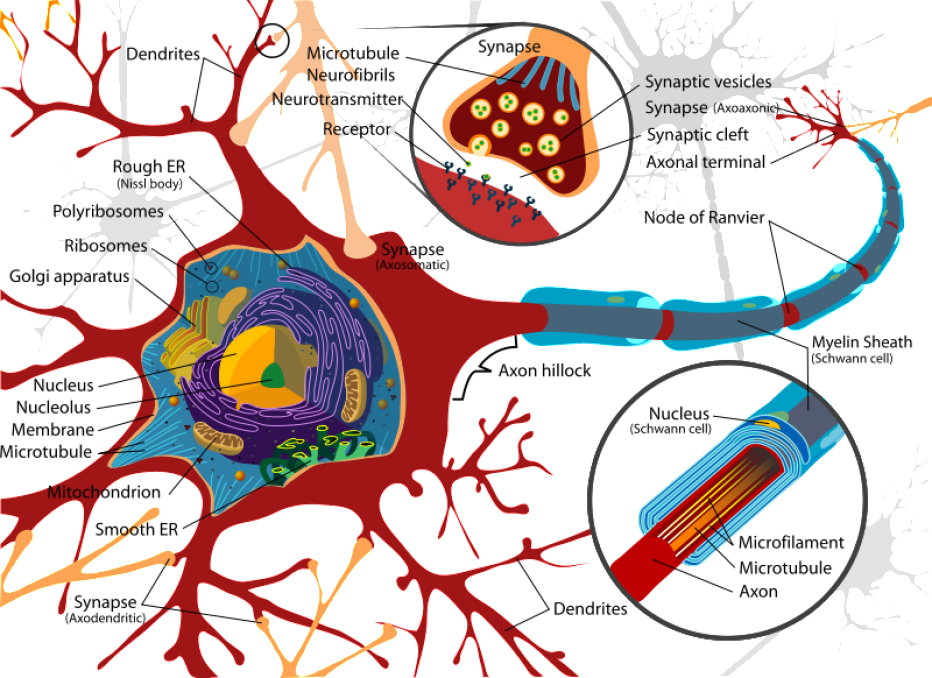
\includegraphics[width=.6\linewidth]{neuron}
  \caption[A neuron. Some shorter caption for the LOF]{A neuron. And some potentially very long caption for an image or table.}\label{fig:sample}
\end{figure}

\section{A}
\kant[6-10]

\section{B}
\kant[11]

\subsection{BA}
\kant[12-14]

\subsection{BB}
\kant[14-16]
Some very important \index{Concept}concept is explained again. See \autoref{tab:sample}.

\begin{table}
  \centering
  \begin{tabular}{lll}
    \toprule
     & A & B \\
    \midrule
    C & 1 & 2 \\
    D & 3 & 4 \\
    \bottomrule
  \end{tabular}\caption[shorter caption]{potentially very long caption}\label{tab:sample}
\end{table}

\subsubsection{BBA}
\kant[16-18]

\subsubsection{BBB}
\kant[18-20]

\section{C}
\kant[20-23]

%%%% %%%%%%%%% %%%%%%%%% %%%%%%%%% %%%%%%%%%
%%%%%%%%% %%%%%%%%% %%%%%%%%% %%%%%%%%% %%%%

% !TEX root = ../main.tex
% !TEX encoding = UTF-8 Unicode
% !TEX TS-program = pdflatexmk
% !TEX spellcheck = en-US
% !BIB program = biber

\begin{savequote}[8cm]
... semantic structure of natural languages evidently offers many mysteries
  \qauthor{--- Noam Chomsky (1965)}
\end{savequote}

\chapter{Background}\label{ch:background}

\minitoc

\section{Introduction}

\kant[10] 

\section{Knowledge Engineering}

\citet{sowa-2000-knowledgerepr} proposed something very important.

In \citep{turing-1948-intelligentmachinery} we/I introduced another important thing.

We/I did other stuff too \citep{turing-1950-computingmachinery}.


Entpropy is a measure for chaos \cite{shannon-1948-entropy}.

Transfer Learning is an important concept \cite{ruder-2019-phdthesis,ruder-2019-transferlearning} which uses deep learning \citep{goodfellow-2016-dlbook}.



%% APPENDICES %%
% Starts lettered appendices, adds a heading in table of contents, and adds a
%    page that just says "Appendices" to signal the end of your main text.
\startappendices
% Add or remove any appendices you'd like here:
% !TEX root = ../main.tex
% !TEX encoding = UTF-8 Unicode
% !TEX TS-program = pdflatexmk
% !TEX spellcheck = en-US
% !BIB program = biber

\chapter{\label{app:1} Additional Material}

\minitoc

THIS IS THE APPENDIX

\par

{ 
  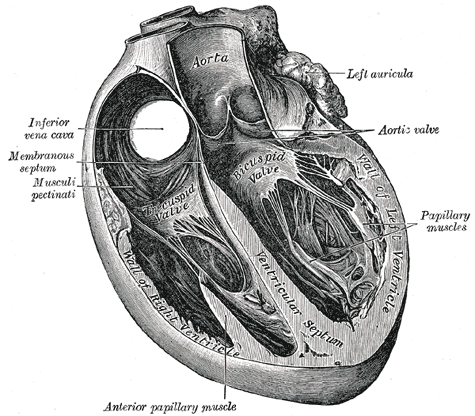
\includegraphics[width=.5\linewidth]{heart.png}
  \captionof{figure}{a heart}\label{fig:heart}
}




%%%%% REFERENCES
% use single-space References
\setlength{\baselineskip}{0pt}
{%
	\renewcommand*\MakeUppercase[1]{#1}%
	% \nocite{*}
	\printbibliography[heading=bibintoc,title={\bibtitle}]
}%

\end{document}
